\documentclass[a4paper]{article}
\usepackage[utf8]{inputenc}
\usepackage[spanish, es-tabla, es-noshorthands]{babel}
\usepackage[table,xcdraw]{xcolor}
\usepackage[a4paper, footnotesep = 1cm, width=20cm, top=2.5cm, height=25cm, textwidth=18cm, textheight=25cm]{geometry}
%\geometry{showframe}

\usepackage{tikz}
\usepackage{amsmath}
\usepackage{amsfonts}
\usepackage{amssymb}
\usepackage{float}
\usepackage{graphicx}
\usepackage{caption}
\usepackage{subcaption}
\usepackage{multicol}
\usepackage{multirow}
\setlength{\doublerulesep}{\arrayrulewidth}
\usepackage{booktabs}

\usepackage{hyperref}
\hypersetup{
    colorlinks=true,
    linkcolor=blue,
    filecolor=magenta,      
    urlcolor=blue,
    citecolor=blue,    
}

\newcommand{\quotes}[1]{``#1''}
\usepackage{array}
\newcolumntype{C}[1]{>{\centering\let\newline\\\arraybackslash\hspace{0pt}}m{#1}}
\usepackage[american]{circuitikz}
\usetikzlibrary{calc}
\usepackage{fancyhdr}
\usepackage{units} 

\graphicspath{{../Calculos-Potencia/}{../Caracteristicas/}{../Consideraciones/}{../Gain-Stage/}{../Input-Stage/}{../Output-Stage/}{../Simulaciones/}{../Alimentacion/}{../Conclusiones/}}

\pagestyle{fancy}
\fancyhf{}
\lhead{22.12 Electrónica II}
\rhead{Mechoulam, Lambertucci, Rodriguez, Londero, Scala}
\rfoot{Página \thepage}

\begin{document}

\subsection{Introducción}

La etapa de salida de un amplificador de audio se encarga de entregar la corriente necesaria a la carga para conseguir la característica de potencia buscada en el amplificador; sin así distorsionar demasiado a la señal, para preservar el THD para la cual se trabajó tanto para disminuir en las etapas anteriores.

Por un lado, se puede utilizar tecnología FET, los cuales no poseen una reducción del "beta" frente a grandes corrientes y por ende una mayor linealidad, a un costo de duplicar el precio de cada dispositivo activo. La otra alternativa, mucho más popular, es usar tecnología BJT. Luego existen varias clases de etapa de salidas distintas, entre ellas A, con una alta linealidad pero muy baja eficiencia; clase B, la cual soluciona el problema de la eficiencia, al costo de la distorsión por crossover; la clase AB, un compromiso entre ambas; variaciones de la popular clase AB, como la clase G que utiliza 4 rieles de alimentación distintos, y muchas más.
En el amplificador de audio diseñado se utilizará clase AB al ser una consideración de diseño.

Dentro de la clase AB existen muchas topologías distintas cada una con sus respectivas ventajas y desventajas. Una de ellas es la topología EF (emitter-follower) compuesta por dos emisores comunes en cascada. En esta configuración, un transistor funciona como \textit{driver}, generalmente situado en un punto Q muy estable. Este transistor proporciona la corriente de base al siguiente, por el cual fluye la corriente que se le entrega a la carga. Dentro de esta topología existen tres tipos mostrados en la Figura (\ref{fig:ef}). En el tipo 1 los resistores de emisor se conectan a la salida. Estos resistores colocan al driver en un punto Q estable. El tipo 2 posee la ventaja de ahorrarse un resistor, colocando uno solo entre los emisores de los transistores. Además, los transistores nunca se polarizarán en inversa al pasar de un semiciclo al otro. En el tipo 3, se conectan los resistores a los rieles de alimentación, lo cual puede mejorar el apagado de altas frecuencias.

%, trim = {0 0 0 20},clip
\begin{figure}[H]
\centering
	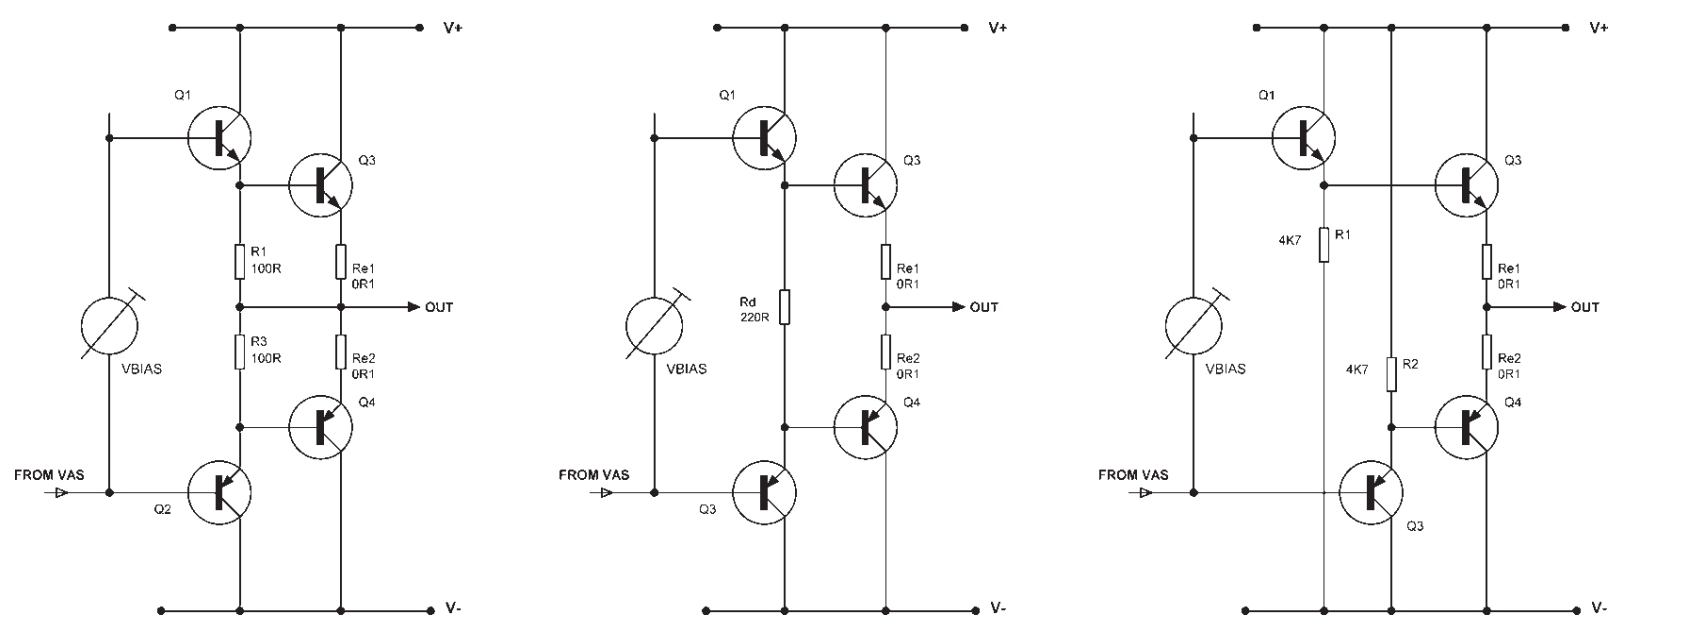
\includegraphics[width=\textwidth]{ImagenesOutput-Stage/pag143-EF.png}
	\caption{Tipos de configuraciones emitter follower. D. Self, Audio Power Amplifier Design Handbook, 5th, p. 143.}
	\label{fig:ef}
\end{figure}


Otra configuración involucra los pares Sziklai, Quasi-Darlington o también llamado par de realimentación, dado que ahora el driver se coloca de manera tal que este compare la tensión a la salida con la entrada, lo cual aumenta la linealidad. Además, como el Vbe del transistor de salida se encuentra dentro del lazo de realimentación, se observa una estabilidad térmica mayor.

%, trim = {0 0 0 20},clip
\begin{figure}[H]
\centering
	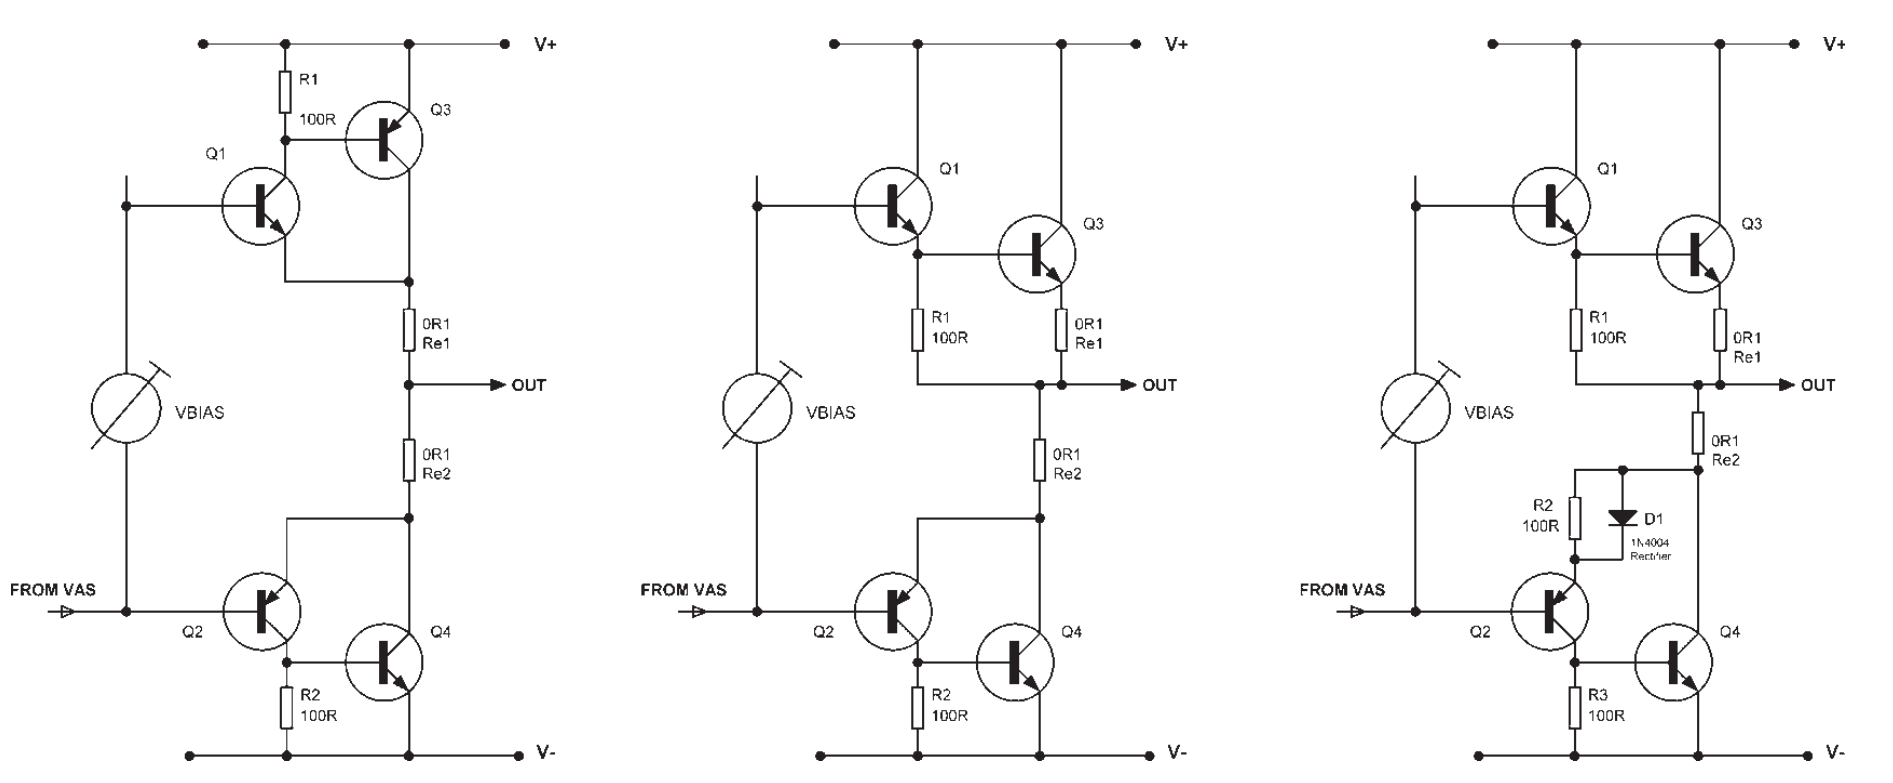
\includegraphics[width=\textwidth]{ImagenesOutput-Stage/pag145-CFP.png}
	\caption{Tipos de configuraciones de par de realimentación. D. Self, Audio Power Amplifier Design Handbook, 5th, p. 145.}
	\label{fig:cfp}
\end{figure}

Una topología la cual en el pasado era casi obligatoria por la falta de transistores PNP de potencia complementarios a los NPN. En esta configuración solamente se reemplaza por un par Quasi-Darlington a los transistores PNP. Esta topología presenta una alinealidad mucho mayor y no será utilizada, aunque existen varios arreglos a la simetría, como por ejemplo utilizando un diodo de Baxandall.

Naturalmente surge al analizar estas etapas de salida la idea de colocar tres transistores en cascada, o más. De ahí surge la topología basada en triples, como la Triple EF. Esta configuración presenta mayor linealidad a alta potencias, un punto Q más estables para los transistores \textit{pre-drivers}, los que proporcionan la corriente a los drivers, debido a que estos manejarán una corriente menor y disiparán menor potencia. Además, al poseer una ganancia de corriente mayor, la etapa de ganancia deberá proporcionar corrientes menores. En la Figura (\ref{triples}) se observan distintas configuraciones triples posibles.

%, trim = {0 0 0 20},clip
\begin{figure}[H]
\centering
	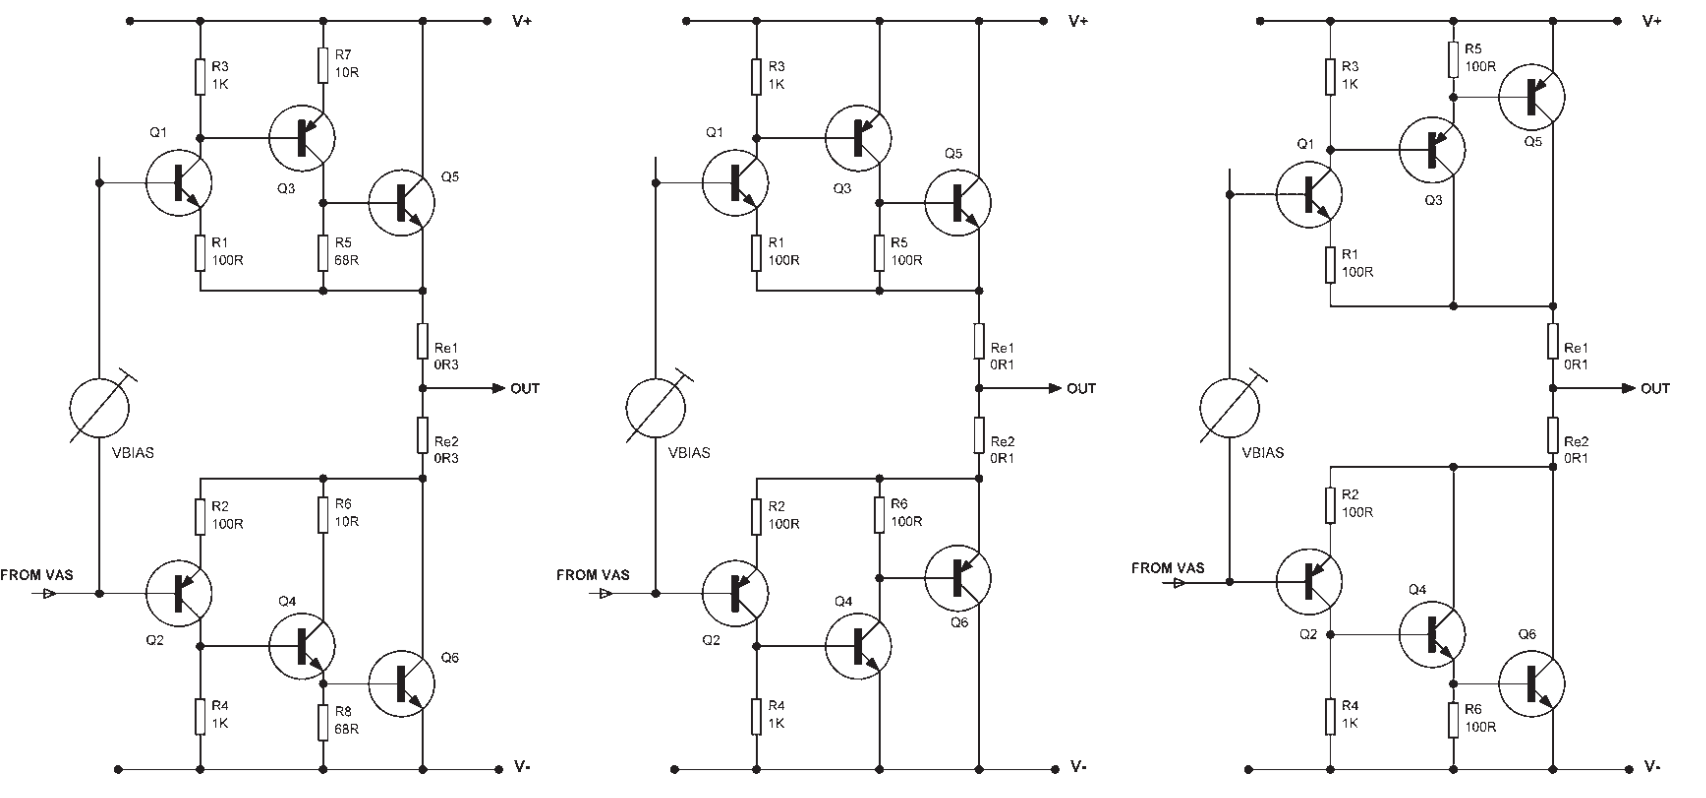
\includegraphics[width=\textwidth]{ImagenesOutput-Stage/pag145-triples.png}
	\caption{Algunos tipos de configuraciones basadas en triples. D. Self, Audio Power Amplifier Design Handbook, 5th, p. 145.}
	\label{fig:triples}
\end{figure}

\subsubsection{Topología Utilizada}


\subsubsection{Generador de Bias}

\subsubsection{Fuente de corriente}

\end{document}